\documentclass{article}

\usepackage[utf8]{inputenc}
\usepackage[T1]{fontenc}
\usepackage{lipsum}
\usepackage{graphicx}
\usepackage{amsmath}
\usepackage[margin=1in]{geometry}
\usepackage{titlesec}
\usepackage{enumitem}

\titleformat{\section}
{\LARGE\bfseries}{\thesection}{1em}{}

\titleformat{\subsection}
{\Large\bfseries}{\thesection}{1em}{}

\begin{document}
\pagestyle{empty}
\section*{Scrum}

\subsection*{Introduzione}
\large
Obiettivi:
\begin{itemize}
    \renewcommand{\labelitemi}{-}
    \itemsep0em
    \item Comprendere come utilizzare e adottare il framework Scrum 
\end{itemize}
\textit{Scrum} rappresenta un insieme di paradigmi utilizzati all'interno di team di sviluppo software, dove l'intento consiste nella creazione di sistemi che abbiano il più alto valore possibile.
Un framework simile è adottato in differenti contesti, ma tramite l'ingegneria del software trova il suo massimo grado di espressione; di seguito è riportata una breve definizione che possa raffigurare l'importanza di uno strumento del genere.\vspace*{14pt}\\
\textit{Definizione informale}\\
Scrum è un framework con cui membri di team di sviluppo possono affrontare problemi complessi in maniera adattiva, approciando ad un comportamento più creativo e produttivo possibile.\vspace*{14pt}\\
Il framework analizzato è spesso associato ad ulteriori metodiche implementative e di stesura del codice, poichè tipicamente il suo utilizzo è attuato per garantire una sequenzialità di pratiche gestionali di sistemi software, per cui adottato in concomitanza di strumenti maggiormente tecnici.
E' fondamentale comprendere che \textit{Scrum} non sia un metodo di sviluppo, ma si concentra solamente sulla pura progettazione della soluzione software dinnanzi ai requisiti funzionali richiesti, per questo spesso è adeguato con altri idiomi di sviluppo del mondo \textit{Agile}, semplificando la realizzazione del prodotto finale.\vspace*{14pt}\\
Ogni progetto che adegua \textit{Scrum} è caratterizzato da iterazioni denominate \textit{sprint}; si riporta una definizione che possa descrivere al meglio l'entità fondamentale su cui si stabilisce l'intero meccanismo.\vspace*{14pt}\\
\textit{Definizione informale}\\
Uno sprint è un'iterazione relegata da una durata predefinita, la quale non può più essere modificata qualora inizializzato il processo esecutivo. Ognuno di essi è preceduto da una riunione organizzativa, in cui si discutono gli obiettivi da portare a termine alla fine del vincolo temporale. In conclusione è ottenuto un prototipo incrementale, oppure meglio definito come \textit{potentially shippable increment}, rappresentante un termine dell'insieme, poichè non dispone di tutte le funzionalità richieste, costituendo potenzialmente una parte della soluzione.

\subsection*{Scrum lifecycle}
\large
In questa sezione è riportata una raffigurazione dell'approccio organizzativo garantito da \textit{Scrum}, in cui sono presenti differenti elementi che ne contraddistinguono la natura, i quali di seguito saranno meglio approfonditi.
\begin{center}
    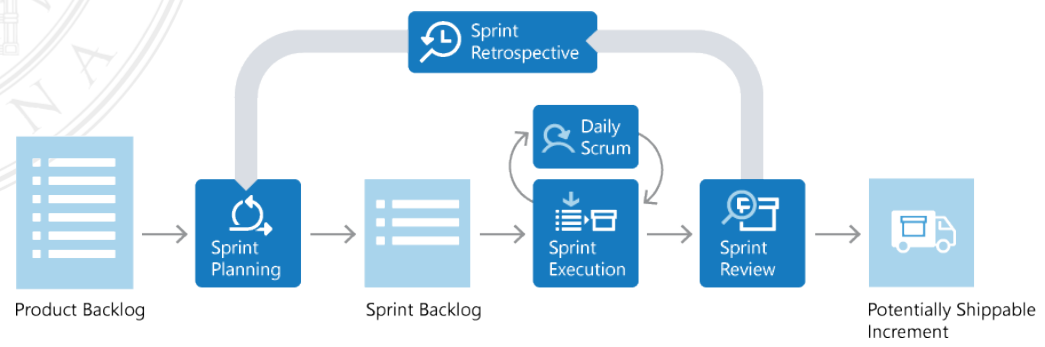
\includegraphics[width=0.8\textwidth]{foto 1.png}
\end{center}
Rispetto alla raffigurazione introdotta, sono stabiliti due insiemi che raggruppano gli elementi illustrati, denominati corrispettivamente \textit{artefatti} ed \textit{eventi}. Di seguito è anticipato l'insieme degli \textit{artefatti}.
\begin{itemize}[label={-}]
    \itemsep0em
    \item \textit{Product backlog} consiste in una lista di \textit{things}, tipicamente ordinata in base all'esigenze del \textit{product owner}, che devono essere riportate all'interno della soluzione software e conseguite, anch'esse suddivise in cinque categorie: \begin{itemize}[label={-}]
                                                                                                                                                                                                                                                                                \item \textit{Requisiti funzionali}, ossia i punti salienti individuati dal team di sviluppo durante le prime fasi di approccio al sistema software, tendenzialemente descritti come \textit{user stories}
                                                                                                                                                                                                                                                                                \item \textit{Bug fixes}, illustrano i \textit{difetti} di cui soffre la soluzione software, si ricorda che un \textit{bug} oppure un \textit{defect} indica un errore logico posto all'interno dell'architettura, il quale non sempre coincide con evidenti \textit{malfunzionamenti}, per cui è necessario adeguare parallelamente allo sviluppo, azioni mirate al \textit{testing} delle funzionalità introdotte
                                                                                                                                                                                                                                                                                \item \textit{Requisiti non funzionali}, interpretabili come un sottoinsieme dei requisiti funzionali ma non fondamentali al conseguimento della soluzione software. In questo ambito sviluppatori devono essere coscienti del \textit{design smell} \textit{needless repetition}, ciò implica che sviluppatori aggiungano layer di funzionalità ulteriori rispetto alle reali pretese degli utenti finali, riportando un erroneo trade-off tra spesa sostenuta e introito ricevuto
                                                                                                                                                                                                                                                                                \item \textit{Requisiti tecnologici}, nuovamente interpretabili come un sottoinsieme derivato dei requisiti funzionali, i quali sono stabiliti come conseguenza della traduzione delle richieste originarie rispetto ad un linguaggio di programmazione che dovrà essere attuato, per cui in relazione anche alle tecniche adoperate pur di conseguire nell'intento
                                                                                                                                                                                                                                                                                \item \textit{Chores}, attività utili per il team di sviluppo, soprattutto in relazione alla decisione di quali strumenti utilizzare, ad esempio realizzare un database relazionale oppure una base di dati No-SQL, azioni che non producono alcun valore aggiunto ma che possono aumentare la produttività interna del team 
                                                                                                                                                                                                                                                                            \end{itemize}
    \item \textit{Sprint backlog} stabilisce un'evoluzione dell'entità che lo procedono, in cui non sono più trattate \textit{user stories}. La \textit{lista antecedente} diviene un insieme di \textit{tasks}, determinate dai membri del team di sviluppo. Le mansioni devono essere concluse entro un certo \textit{sprint}, per cui ad ognuna di esse è associato un valore, espresso in ore richieste per completare lo specifico compito, obbligatoriamente minore di un giorno lavorativo; qualora \textit{task} siano associate ad un valore maggiore occorre suddividerla in due differenti mansioni 
\end{itemize}
Definita la categoria di \textit{artefatti}, successivamente sono descritti gli \textit{eventi} che caratterizzano \textit{Scrum}.
\begin{itemize}[label={-}]
    \itemsep0em
    \item \textit{Sprint planning} è un evento in cui il \textit{product owner} definisce un obiettivo e presenta, in relazione al team di sviluppo e all'intento che voglia essere conseguito, quali temi siano caratterizzati da una maggiore importanza all'interno del \textit{calderone}, ossia il \textit{product backlog} di riferimento, ed ad ognuno di essi è associato il valore temporale necessario, previa precedente discussione, per compiere la \textit{user story}, divenendo un \textit{task}, affinchè sia popolato \textit{sprint backlog}
    \item \textit{Daily scrum} raffigura un incontro tra i membri del team di sviluppo, tendenzialmente di breve durata, in cui si discutono e si analizzano velocemente i progressi implementativi attuati fino ad un determinato momento. Ciò accade giornalmente, indipendentemente dalla difficoltà delle \textit{tasks} e dallo stato di avanzamento della soluzione, potrebbe inoltre rappresentare un'occasione utile in cui si manifestano perplessità e problematiche inerenti allo sviluppo 
    \item \textit{Sprint review e Sprint retrospecting}, al termine di uno \textit{sprint} sono attuate due differenti operazioni, suddivise in: \begin{itemize}[label={-}]
                                                                                                                                                    \itemsep0em
                                                                                                                                                    \item \textit{Review}, consiste nell'analisi del prototipo software realizzato, rispetto al \textit{goal} definito dal \textit{product owner}, affinchè sia possibile osservare se risulti essere idoneo alla prospettiva iniziale, o più semplicemente se in grado di produrre il comportamento atteso. Partecipano tutti i membri del \textit{team di sviluppo} e i \textit{portatori di interesse}, in maniera tale che sia imbastita una discussione del prodotto realizzato, ottenendo il livello di compatibilità con l'aspettative degli utenti finali
                                                                                                                                            \item \textit{Retrospecting}, consiste in un'\textit{analisi interna}, in cui sono coinvolti il \textit{Scrum Master} e ogni membro del \textit{team di sviluppo}, dove il tema centrale consiste nell'analisi dell'approccio adeguato in relazione all'obiettivo originario, permettendo di descrivere quali entità siano conformi all'ambiente di sviluppo e quali dovrebbero subire delle modifiche in modo tale che risultino affini al gruppo software
                                                                                                                                                \end{itemize}
\end{itemize}

\subsection*{Scrum Roles}
\large
Trattandosi di un'idioma sviluppato per favorire e semplificare la complessità progettuale, al suo interno sono stabiliti una serie di ruoli conformi all'intento di \textit{Scrum}, in cui si contraddistinguono:
\begin{itemize}[label={-}]
    \itemsep0em
    \item \textit{Product Owner}, figura indispendabile all'interno di tematiche relative all'implementazione di sistemi software, poichè rappresenta il \textit{costumer}, ossia colui che richiede a team di sviluppo di adeguare le proprie richieste ad un meccanismo automatizzato. Trattandosi di una figura esterna all'effettività descritta, si occupa sostanzialmente di definire le \textit{priorità}, le \textit{scadenze} ed infine le \textit{funzionalità} che la soluzione debba possedere
    \item \textit{Scrum Master}, il responsabile della corretta applicazione dei principi e pratiche di strumenti \textit{agile}, promuove attività di supporto ai membri del team in difficoltà coordinando ed assegnando differenti metriche di implementazione, inoltre è garante del totale rispetto dei limiti temporali imposti dagli \textit{artefatti} ed \textit{eventi}, tipicamente organizzando riunioni e promuovendo la discussione tra sviluppatori affinchè siano condivise perplessità e problematiche, favorendo in tal modo il trasferimento di conoscenza
    \item \textit{Development Team}, team di sviluppo composto da un limite minimo di cinque membri fino ad un totale di nove, qualora siano sviluppati progetti di piccola o media dimensione; la scelta di una cardinalità simile avviene per garantire scalabilità informativa, dato che il gruppo è responsabilizzato per la realizzazione del prodotto finale e può contare solamente su capacità e conoscenze interne pur di proseguire corettamente con l'implementazione
\end{itemize}
\end{document}